\chapter{Directed module detection in a large-scale expression compendium}\label{ch:distiller}
\chaptermark{Gene coexpression module discovery}


\instructionsintroduction

% specially indented text in bold 
\newcommand{\distsubparagraph}[1]{\hspace{-2mm}\textsf{\textbf{#1}}}


\section{Introduction}

Omics based approaches are increasingly being used to uncover underlying mechanisms of bacterial behaviour \cite{Fierro2008}. The obligate deposit of high throughput experiments in public databases upon publication has tremendously increased the amount of publicly available experiments. Mining these data sources helps in gaining a global condition dependent view on bacterial gene regulation \cite{Lemmens2009, Fadda2009}, in expanding the current knowledge on transcriptional interactions with novel reliable predictions \cite{Faith2007, Ernst2008}, and in comparing transcriptional networks across species \cite{Fierro2008, Babu2009}. It also offers molecular biologists the possibility to see their own dedicated analysis in light of what is already available. Inferring transcriptional networks from these public data usually requires complex normalization procedures \cite{Faith2008} and computationally intensive algorithms. To enhance the usability of these tools, they are often wrapped in a web service.

In this chapter, we will illustrate how compendia of public expression data can be used to identify condition dependent coexpression modules, in which a particular gene of interest is involved (`directed' module detection), by means of two web services: COLOMBOS \cite{Engelen2011} and DISTILLER \cite{Lemmens2009} (the latter in combination with the visualization tool ViTraM \cite{Sun2009}). Figure \ref{fig:workflow-distiller-colombos}illustrates the difference between both approaches. COLOMBOS only relies on expression data to retrieve condition dependent modules, implying that there is a functional relationship between the module genes, but not necessarily that they are regulated by the same (set of) transcription factor(s). DISTILLER, in contrast, incorporates additional motif data and the constraint that module genes should share the same regulatory program, implying that the module's condition dependent coexpression can be directly linked to transcriptional coregulation. 

To clearly demonstrate the functionalities of these web services, the gene \textit{sodA} is used as a case study. This gene encodes for a protein with superoxide dismutase activity, which reduces harmful free radicals of oxygen formed during normal metabolic cell processes \cite{Fawcett1995, Tardat1993, Jair1995}. It is known to be regulated by several regulators, such as, Fur, SoxS, and MarA. As such its expression is coupled to different biological conditions: multiple antibiotic resistances (MarA), superoxide resistance (SoxS) and the intracellular iron pool (Fur). By applying different analysis approaches (COLOMBOS and DISTILLER), we will show how to identify \textit{sodA} containing modules, i.e. genes that behave similarly to \textit{sodA} in a condition dependent way from large-scale expression compendia.

\begin{figure}[tb]
	\centering
  	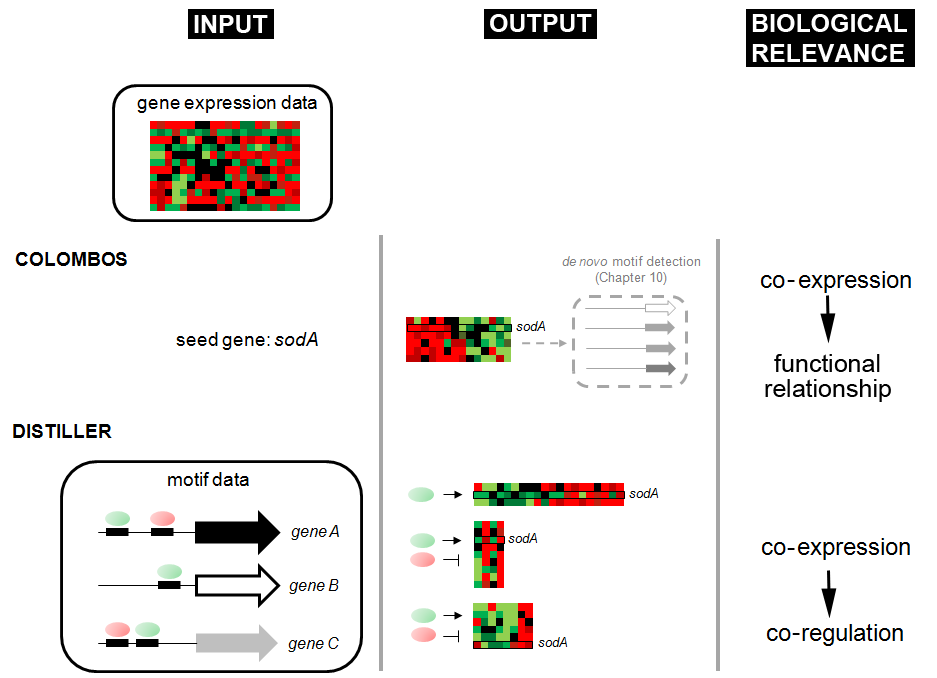
\includegraphics[width=1\textwidth]{Fig1-Workflow-figure.png}
	\caption[Workflow of directed module detection in expression 
	compendium]{
	\textbf{Workflow of different methods for the directed module detection in 
	expression compendium.} 
	Coexpression modules are detected by COLOMBOS starting from a user provided 
	seed gene (e.g., \textit{sodA}). 
	DISTILLER searches for coexpression modules in a global fashion 
	(information on seed genes is not a prerequisite) and is constrained by 
	regulator-to-gene assignments. 
	Coexpression patterns retrieved by COLOMBOS point toward a functional 
	relationship among the module genes but do not necessarily imply 
	coregulation. To gain insights on the regulatory program of those genes, de 
	novo motif detection tools could be applied to analyze their promoter 
	regions. Inherent to the regulator-to-gene constraints implemented in 
	DISTILLER, there is a direct link between coexpression and coregulation for 
	the genes in the modules that it retrieves.}
	\label{fig:workflow-distiller-colombos}
\end{figure}




\section{Material}

\subsection{Cross platform expression compendium}\label{sec:dist-comp} 

An expression compendium is essentially an organism-specific matrix of expression values derived from publicly available microarray experiments which are homogenized to make them comparable. The rows of the matrix correspond to the known genes of the organism in question. Each column is a \textit{contrast} defined as a comparison between two different biological samples, one acting as a test and the other as a reference. The expression values are calculated as expression log-ratios representing gene expression changes induced by the difference between samples. Relative expression calculated intra-experiment/platform (i.e. between two conditions measured in the same microarray experiment using one platform) negates much of the platform and experiment specific variations that makes it impossible to reliably compare the absolute quantities reported in different experiments \cite{Shi2006}. The extensive annotations are manually curated for each contrast, specifying which aspect(s) (experimental conditions) has/have been changed between the test and reference samples. The methodology utilized to create such a compendium is explained in details in Chapter \ref{ch:command}.

The \textit{Escherichia coli} compendium used in here contains 1429 condition contrasts obtained from 1747 microarrays of 84 experiments across 35 platforms, covering the expression profiles of 4295 genes under various conditions annotated by 242 different condition properties grouped under 56 condition ontology terms. Furthermore, several sources of gene information from main curated databases are integrated into the compendium as well, such as, the pathway and operon information from EcoCyc \cite{Keseler2009}, the Gene Ontology annotation from UniProt GOA \cite{Camon2004}, and the regulon information from RegulonDB \cite{Gama-Castro2008}. (see Table \ref{tab:colTB-overview}) 

\subsection{Coexpression modules}

Genes that have the same regulatory program (here defined as having the same transcription factor binding motifs in their promoter regions) behave similarly: their expression responds in a similar manner to certain alterations in the organism's intra- or extracellular environment. This is called \textit{coexpression}. The evidence of coexpression points to a functional relationship between coexpressed genes, and might sometimes be an indication of shared regulatory programs.  Such a functional relatedness is only enforced when coexpression occurs across multiple different conditions. Since each value in our data set does not represent an absolute measure of expression, but rather a relative one associated to a contrast (test versus reference), coexpression in this case translates to genes showing log ratios that are significantly different from zero for at least one condition contrast, and for each of the involved contrasts show coherent changes in the same direction (either up or down). The methods, COLOMBOS and DISTILLER, demonstrated in this chapter employ different computations to score this coexpression, but essentially look for the same phenomenon.

Genes are only coexpressed under certain condition contrasts. This combined set of genes and condition contrasts, where the coexpression pattern appears, is what we refer to as a \textit{module}. Extra constraints can be used to tune the module concept for specific purposes. For example, extra requirements could be added that genes in the module should have (known) motif(s) in common.


\subsection{COLOMBOS}

COLOMBOS, an acronym for \textit{COLections Of Micrcroarrays for Bacterial OrganismS}, is a web service \cite{COLOMBOS, Meysman2014} (Figure \ref{fig:colombos}) for interactively exploring, querying, analyzing and visualizing data from cross platform expression compendia through an intuitive interface. Currently it provides the possibility to query expression compendia based on the annotation of their contrasts and/or genes. This service can be used, for instance, to search for genes being coexpressed with one or more genes of interest under a pre-specified set of condition contrasts, or to search for the condition contrasts in an expression compendium under which a pre-specified gene set is coexpressed. As such, it can identify coexpression modules based on user input. In COLOMBOS, modules can be visualized as interactive heatmaps, showing the annotation of genes and condition contrasts as obtained from public databases and corresponding literature. More details of COLOMBOS are discussed in Chapter \ref{ch:colombos}.

\begin{figure}[tb]
	\centering
  	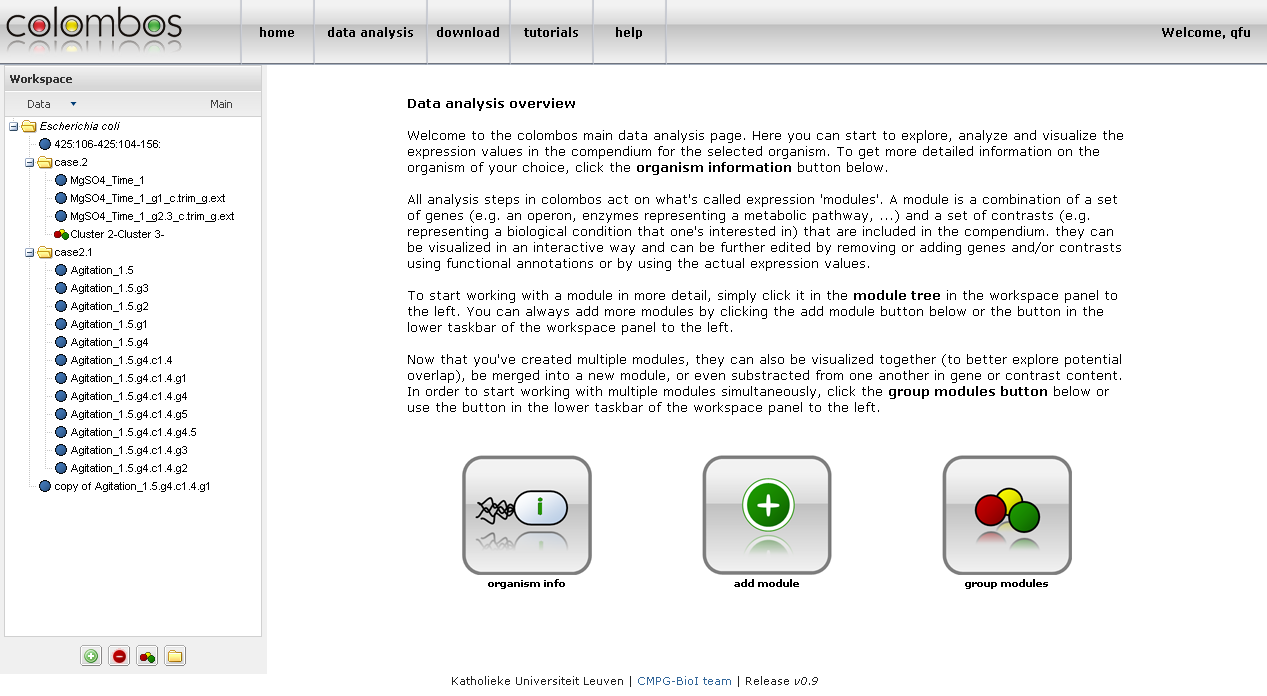
\includegraphics[width=1\textwidth]{Fig2-COLOMBOS.png}
	\caption[COLOMBOS web service interface]{\textbf{COLOMBOS web 
	service interface.} 
	The interface is composed of three parts: the website navigation header at 
	the top, the workspace (showing a module tree) at the left-hand side, and 
	the operating space (here showing the `Data analysis overview' panel) 
	filling the center.}
	\label{fig:colombos}
\end{figure}

Currently COLOMBOS (v2.0) runs on three browsers: Firefox, Google Chrome, Safari, and Opera. Be sure that you are using the latest version of the browser to have the best compatibilities. Please check the website for updated information.

\subsubsection{COLOMBOS expression data format}\label{sec:dist-format-col}
To use COLOMBOS requires no input file, as the expression compendium is an integrate part of It.   It does provide a tab delimited ASCII file format for expression data export, containing information on the user created module consisting of a particular set of genes and the corresponding set of contrasts under which these genes are coexpressed. There are two sections in this file. The first one describes the condition information of the module. It specifies for each contrast the name and description of its test and reference sample, the corresponding experiment identifier, the online database from which the experiment was retrieved, the microarray platform used to measure the sample hybridizations, and finally, the annotated condition changes between the test and the reference sample. The second section contains three parts: the corresponding contrast identifiers in the first row; the gene information (gene locus tag, gene name, and internal gene identifier) in the first three columns; and the expression log-ratios of the compendium. Starting from the $4^{th}$ column, each column in the file corresponds to one condition contrast. Each of the rows represents one gene and its expression values for different condition contrasts. 

\subsection{DISTILLER}\label{sec:dist-distiller}
DISTILLER (\textit{Data Integration System To Identify Links in Expression   Regulation}) is a data integration framework that searches for condition dependent transcriptional modules by combining expression data with information on the interaction between a regulator and its corresponding target genes, for instance based on motif screening. A module is here defined as a set of genes coexpressed under a sufficiently large number of conditions and sharing the motif instances of the same regulator(s).  The expression data used by DISTILLER could be either absolute expression values or log-ratios.

DISTILLER searches the modules in a global fashion over the entire dataset through three steps: identification candidate modules, module filtering, and module extension. Built on advanced itemset mining approaches, it first exhaustively enumerates all possible valid \textit{closed} modules (see next Section) as candidates. The candidates are partially redundant as they might share the same genes or condition contrasts. Therefore, in the filtering step, modules are prioritized by calculating an interest score for each of them.  The score takes into account the probability that a module of the same size can be found by chance in the input dataset, whereas, at the same time, penalizes the overlaps between modules. The resulting top ranking modules are statistically significant yet distinctive. These initial modules obtained under stringent thresholds are called `\textit{seeds}', in which the identified interactions between a transcription factor and its target genes are highly reliable (high precision).  However, some true interactions might be missed (lower sensitivity). Hence, in the last module extension step, the modules retained after filtering are further extended with additional genes by applying relaxed thresholds on minimal coexpression level and motif score. Note that it is not required to execute all three steps.  The result of each step can be analyzed and visualized independently.

The DISTILLER web service \cite{DISTILLER} (Figure \ref{fig:distiller}) is  designed to leverage the difficulty of applying the algorithm by providing an  easy-of-use and consistent interface that links all three steps together.  The interface is separated into two sections vertically. The information panel at the top provides a brief explanation of the site's functionality. The project panel at the bottom is where the user interacts with the site. It is further divided horizontally into three sections.  At left, the `Project Information' panel provides information of the current project and the links to access the input, output, and log files. The `Operation' panel at the center is where a user runs DISTILLER algorithm. It has three tabs, each of which provides access to one step of the algorithm, namely, module detection, module filtering, and module extension. The explanation for the parameter settings and the input data file format (if required) of the corresponding step selected in the `Operation' panel are provided in the `Online help' panel at right for your reference.   The website works properly on Firefox and Google Chrome.  Efforts are undertaken to make it compatible with other browsers as well.  Please check the website for updated information. 

\begin{figure}[tb]
	\centering
  	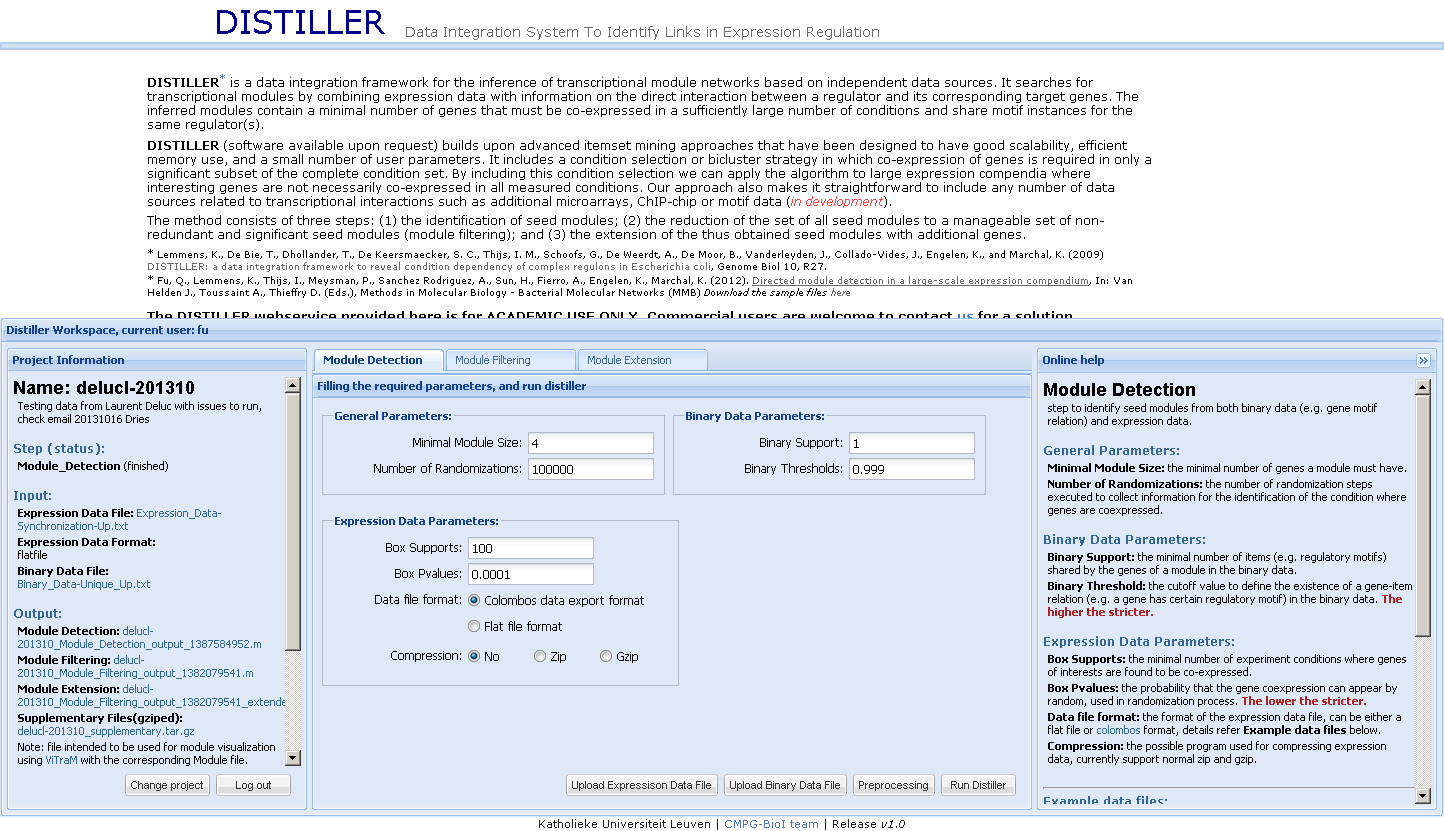
\includegraphics[width=1\textwidth]{Fig3-DISTILLER.png}
	\caption[DISTILLER web service interface]{\textbf{DISTILLER web service 
	interface (at module detection step).}}
	\label{fig:distiller}
\end{figure}

For this case study, the data consist of the same compendium as the one accessed through the COLOMBOS website. Hence, the columns of the expression matrix, across which DISTILLER defines coexpression, correspond to the condition contrasts as defined in the compendium (see Section \ref{sec:dist-comp}). 

\paragraph{Closed module}
A module is considered \textit{closed} if it cannot be further extended by any other gene without reducing the number of motifs shared by all of its genes. To search such a candidate, the algorithm \cite{Lemmens2009} starts with the smallest module that contains only one gene, and gradually extends them by merging with other modules. A candidate is found when any extension violates the conditions implied by `closed'.  Only closed modules that contain the minimal number of motifs and condition contrasts are considered valid. % (meet the required minimal Supports on the motifs and condition contrasts)



\subsubsection{DISTILLER input file format}\label{sec:distiller-infile-format}
DISTILLER requires two input files: an expression data file and a motif data file. In the case study described here, the expression data file contains the expression log-ratios for each gene under each contrast.  Two possible input formats are allowed for the expression data file.  The first one is a matrix based flat file format with header, in which, the first row contains the identifiers of each contrast, each subsequent row corresponds to a gene, each column represents a contrast.  Gene name is used to specify a gene in the first column of each row. The second format is that of the COLOMBOS expression data export file (see Section \ref{sec:dist-format-col}).   The system further supports the use of two most common compression formats to handle the large data set, namely, Zip\footnote{In case of zip file, the system allows only one file in the compressed file that is the input expression data file. An error is generated when this condition is violated.} and Gzip.

The motif data file contains the results of a motif screening analysis \cite{Hertzberg2005}.  Each motif screening score indicates the probability that a motif instance is present in the promoter region of a gene, with 1 as the maximum score and 0 the minimum. The data is specified in a text file containing a data matrix with header, in which the header are motif names, the row corresponds to gene, and the column represents the motifs screened.  Similarly to the expression data, except for the header, each row starts with gene name specifying the corresponding gene.

Additionally, users can provide an operon information file that will be used during the module extension step.  It contains two items in each row, the gene that belongs to an operon, and an identifier of that operon.

In DISTILLER, the different data files are coupled in the gene direction, so the user should make sure that the same gene identifiers are used in each file, although the order of the genes need not to be the same.


\subsubsection{DISTILLER output file format}\label{sec:distiller-outfile-format}
All three steps of DISTILLER output the results in the same format: a `.m' file. It contains the information of the identified modules, with each module described in a section, separated by an empty line.   Each section contains four data fields.  Given a section specifying the information for a module $M$, the field `Significances' holds the $p$-values that were assigned to $M$ by the itemset mining algorithm \cite{Zaki} utilized by DISTILLER.  The field `items' contains the information of the genes that belong to $M$, each of which is represented by its row number\footnote{When   counting the row number of a given gene, there are certain caveats. First, the   header should not be counted.  Second, the count should start from 0. Hence   the first row is of row number 0 instead of 1.} in the expression data input file. The field `boxtidset1' specifies the contrasts of $M$, in which the genes in $M$ are coexpressed, each of which is represented by its column number\footnote{To count the column number referred in the `.m' file, the first   column containing gene information should not be counted, and it starts at 0.} in the expression data input file. Finally, the field `tidset1' contains the motifs of $M$ shared by its genes, specified by their column numbers in the motif data input file.   Each module is represented by a unique number indicated between the `\{\}' brackets after the name of each corresponding data field.

Besides the main output file, two supplementary files required to use the visualization software ViTraM are also provided. They are bundled in a compressed file that can be downloaded from the website. The file whose name starts with `expdata\_' contains the preprocessed input expression data, and the other starting with `binary\_' contains the preprocessed input motif data. The file formats of these two files are the same as the corresponding input files described in previous Section. 

\paragraph{Output notification email}\label{sec:distiller-email}
Since each step of DISTILLER may take hours or even days to finish, the result is sent to the user by email. This notification email is of a standard format, with subject `DISTILLER process result notification email'. On the first line, the information about the finished process and the corresponding user project is presented, followed by the link to the result file, then the link to the supplementary file bundle required for visualization.




\subsection{ViTraM}\label{sec:dist-vitram}
To analyze DISTILLER output, we use ViTraM (\textit{VIsualization of TRAnscriptional Modules}) to visualize overlapping transcriptional coexpression modules together with the motif information in an interactive way. Here, we will only briefly discuss this tool. For more details we refer to \cite{Sun2009}.

ViTraM 2.0 is used for this case study (download at \cite{ViTraM}).  Written in JAVA, it can run under any platforms with JAVA support.  On Windows ViTraM comes with two options: vitram\_Windows\_512M.bat or vitram\_Windows\_2G.bat. The former has a minimum memory requirement of 1Gb RAM.  And we advise to use a computer with at least 3Gb RAM to run vitram\_Windows\_2G.bat. 


\subsubsection{ViTraM input file format}
ViTraM requires an XML file and an expression file as input. The XML file contains the information of the transcriptional modules that will be visualized: the genes and conditions composing the modules and additional information such as motifs that are assigned to modules by DISTILLER. Due to the complexity of the XML format, an extra tool called XMLCreator is available at the ViTraM website to automatically generate the XML file from the DISTILLER output file (see Section \ref{sec:distiller-outfile-format}).  Conveniently, the tool also generates a smaller expression data file containing only the relevant expression values from those genes and condition contrasts existing in the result modules obtained by DISTILLER.  Moreover, the tool can also incorporate extra information into XML file, for example, the motif data contained in the binary supplementary file mentioned in Section \ref{sec:distiller-infile-format}. For the purpose of this study, we will not discuss this XML file format in detail.  Interested users can find more information in \cite{Sun2009}.



\subsection{Sample files}\label{sec:dist-sample}

The following four sample files are provided as example input files for this case study. The file expdata\_COLOMBOS\_module\_information.txt is an example of the exported module data file of COLOMBOS, which, as one of the input formats of the expression data for DISTILLER, contains both the gene and condition contrast information, and the log ratio expression data. The file expdata\_DISTILLER\_Expression.txt is an example of the other expression data format accepted by DISTILLER. The file binary\_DISTILLER\_Motif.txt is the motifdata containing motif scores for each gene. And finally, the file operon\_DISTILLER\_OperonGenes.txt is the example operon information file.

Furthermore, three example output files, corresponding to the output generated after each step of DISTILLER, are provided. DISTILLER\_Output.m is the output of the seed module identification step, DISTILLER\_FilteringOutput.m is the output of the module filtering step, and DISTILLER\_outputExtended.m is the output of the module extension step. Files expdata\_DISTILLER\_supple.txt and binary\_DISTILLER\_Motif\_supple.txt are provided as the supplementary files used for visualizing modules contained in those sample output files.

Finally, ViTraM\_Modules.XML is provided as the XML file describing the modules, and ViTraM\_Expression.txt is provided as the expression data file used by ViTraM.

One can download all the example files from here \cite{DISTILLER-sample} or at the DISTILLER website \cite{DISTILLER} (follow the sample file link of the second references).






\section{Methods}

We will describe the steps required to use two web services, COLOMBOS and DISTILLER, to identify coexpression modules around a (set of) gene(s) of interest (query genes). This will be illustrated by applying them to the query gene \textit{sodA} as a case study.   The analysis flow based on COLOMBOS shows how it can be used to search for genes that are coexpressed with a (set of) query gene(s) under the human guidance.  Alternatively, the DISTILLER approach, combining expression and motif data, detects coexpressed and coregulated gene sets across the whole data set in a single run in an unsupervised way.


\subsection{Identifying coexpression modules using COLOMBOS}\label{sec:dist-module-colombos}

To search for coexpressed genes using COLOMBOS, we will first create an initial expression module by specifying a set of genes of interest (query genes), and use COLOMBOS to extract the most relevant contrasts, where the chosen genes are differentially expressed.  Next, the module is extended with genes that are coexpressed with the initial gene set under the selected of contrasts. Here, we explain this workflow starting with a single query gene, \textit{sodA}.


\subsubsection{Create the initial module}

\begin{small} % Step 1

\paragraph{Step 1} 
Go to COLOMBOS website \cite{COLOMBOS}, and create the initial module based on the known gene set of interest and the biological conditions that are known to affect these genes when changed.

\subparagraph{Step 1.1}	To start the analysis, click on `data  analysis' in the title bar (Figure \ref{fig:colombos}) to bring up the data operation interface in the center part of the website.  It is separated horizontally into two parts. At the left hand side, there is a `workspace' information panel that lists all the modules created in a tree structure. This panel is always visible when residing on the data analysis page. Since no module has been created, it is currently empty. The other part of the page, referred as the operating space in this text, is where the visualization and analysis of the expression data takes place and is currently occupied by the `Data analysis overview' panel (hereafter referred to as `overview panel'). This panel serves as a intuitive guide showing the available analysis options depending on the current workspace state along with some brief explanations.\vspace{1.5mm} Since we just started a new session, there is only one button `select organism' available. Click it, and select the organism `\textit{Escherichia coli}', which this case study focuses on. Notice now this species appears in the workspace panel as the root of the tree.


\subparagraph{Step 1.2}	After the species is picked, the content of the  overview panel is changed accordingly. The button `select organism' is replaced by two other buttons `organism info' and `add module'. To create our initial module for \textit{sodA}, we click the `add module' button to bring up the `Add module overview' panel. In this panel, there are three buttons `select gene only', `select contrasts only', and `select gene and contrast'.  Each corresponds to a different method for creating a module. Here, we utilize the first option to manually specify the query gene \textit{sodA} and let the system automatically identify the most relevant contrasts for it based on expression data. Clicking `select gene only' brings up the gene selection panel at center.  Four available options are available: `By gene name/locus tag', `By transcriptional regulation', `By pathway', and `By transcription unit'. The first option allows us specify gene manually. Click the yellow box surrounding the text `By gene name/locus tag', fill in `\textit{sodA}' in the text box appeared (one gene per row), and then click the `Done' button to proceed.

\subparagraph{Step 1.3}	

\begin{figure}[b]
	\centering
  	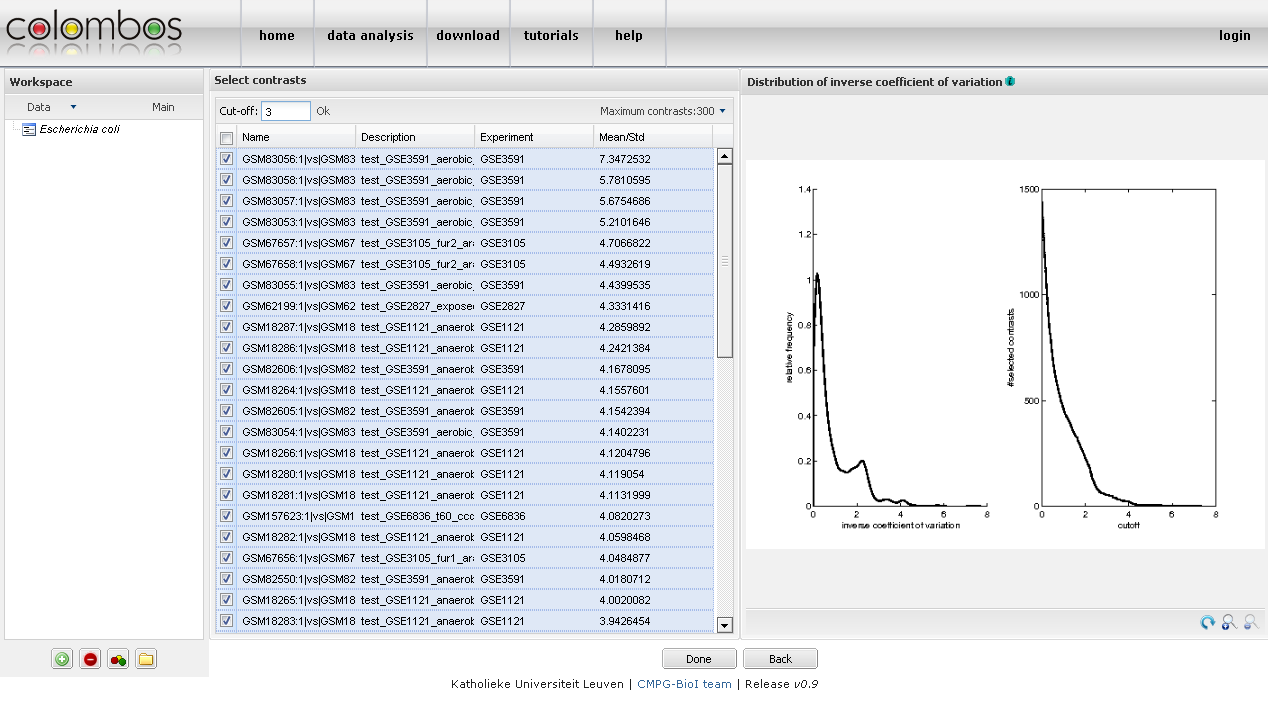
\includegraphics[width=1\textwidth]{Fig4-Condition-contrasts-ranking-panel.png}
	\caption[COLOMBOS contrast ranking interface]{\textbf{The `ranked contrast 
	selection' interface to choose contrasts based on the specified module 
	genes (\textit{sodA} in this particular case).}}
	\label{fig:colombos-ranking}
\end{figure}

After specifying the genes, a `ranked contrast selection' panel (Figure \ref{fig:colombos-ranking}) appears in the operating space, which allows the user to select contrasts ranked by a score that prioritizing those show the highest magnitude of change and most coherent coexpression for the selected set of genes (see Appendix \ref{apd:contrast-score}). The panel is separated into two parts horizontally.  At the left, the contrasts are ranked according to the score from highest till the lowest. A cutoff value can be specified in the box above the list to select only those with higher scores. The figures to the right show, from left to right, a density plot showing the distribution of the scores across the whole compendium and a plot showing the number of contrasts that will be added if a given cutoff is selected.  There is no absolute guideline to choose the cutoff. Several try-outs may be needed to identify the optimal one.
\\
For our initial module, we chose cutoff value 3. Specify it, and click `Ok' button at the side. The contrast list is then filtered, and all that left in the list are automatically selected to be added to the module. Click `Done' button at the bottom, and fill in `sodA\_c3' as the module name to create our initial module.  The newly created module appears in the module tree in the workspace as a node directly under the root (presenting the selected organism \textit{Escherichia coli}).


\end{small} % Step 1



\subsubsection{Inspect the existing modules}

\begin{small} % Step 2
\paragraph{Step 2} One can review the information of a module through various options.

\subparagraph{Step 2.1}	Click the module you want to check in the workspace to show its overview tab (Figure  \ref{fig:colombos-init-module}) in the center. The tab shows on top a brief summary of the module, including, name, description, number of genes and contrasts it contains, as well a list of significantly enriched Gene Ontology (GO) terms of class biological process ($p$-values $< 0.1$, details see Appendix \ref{apd:enrichment}) for the module genes. At the bottom, there are four buttons to \textit{visualize}, \textit{edit}, \textit{split}, or \textit{delete} the module. The function of \textit{visualization} and \textit{delete} is straightforward. The \textit{edit} function allows user to modify either the genes or the contrasts of the module. Instead, the \textit{split} function breaks the current module into several new ones by separating either its genes or its contrasts into distinctive groups and creating a module for each selected group. 

\begin{figure}[tb]
	\centering
  	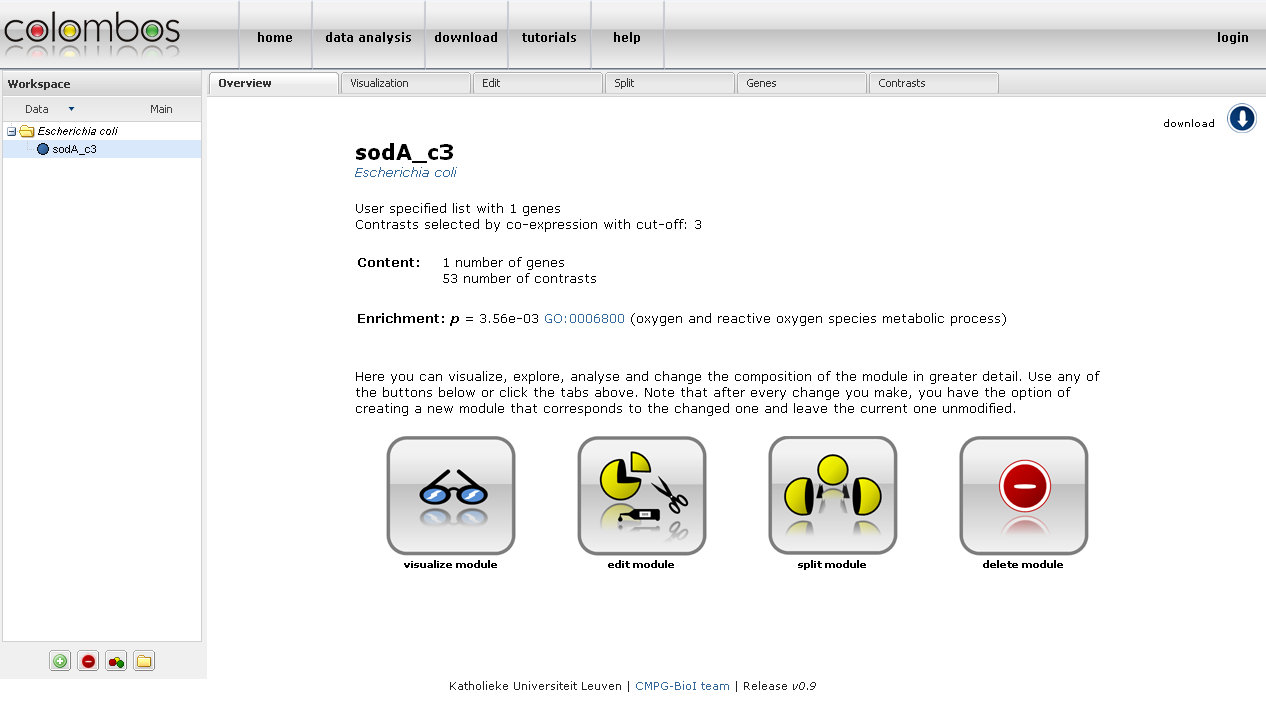
\includegraphics[width=1\textwidth]{Fig5-Module-overview.png}
	\caption[`sodA\_c3' module overview]{\textbf{The overview tab of 
	the module `sodA\_c3'.}}
	\label{fig:colombos-init-module}
\end{figure}


\subparagraph{Step 2.2}	Each module can be visually presented as a heatmap. In it, each square represents one gene's expression log ratio for a certain condition contrast. A red color indicates over-expression while a green one shows under-expression. The intensity of the color corresponds to the magnitude of the expression change. The brighter the color, the higher the absolute ratio value. To view the heatmap, click `Visualization' button in overview tab to switch to heatmap tab.  The heatmap is shown at the center with an information panel at the right. Hovering over the heatmap, the information of the gene and the contrast under the cursor will be shown in the information panel. Various options exist to group the contrasts in the heatmap according to their experiments, condition properties, and the associated condition ontology terms. They can be selected from the dropdown box located at the lower left corner of the tab. The heatmap of our module sorted on condition ontology is shown in Figure \ref{fig:colombos-heatmap-m1}.
%
\begin{figure}[tb]
	\centering
  	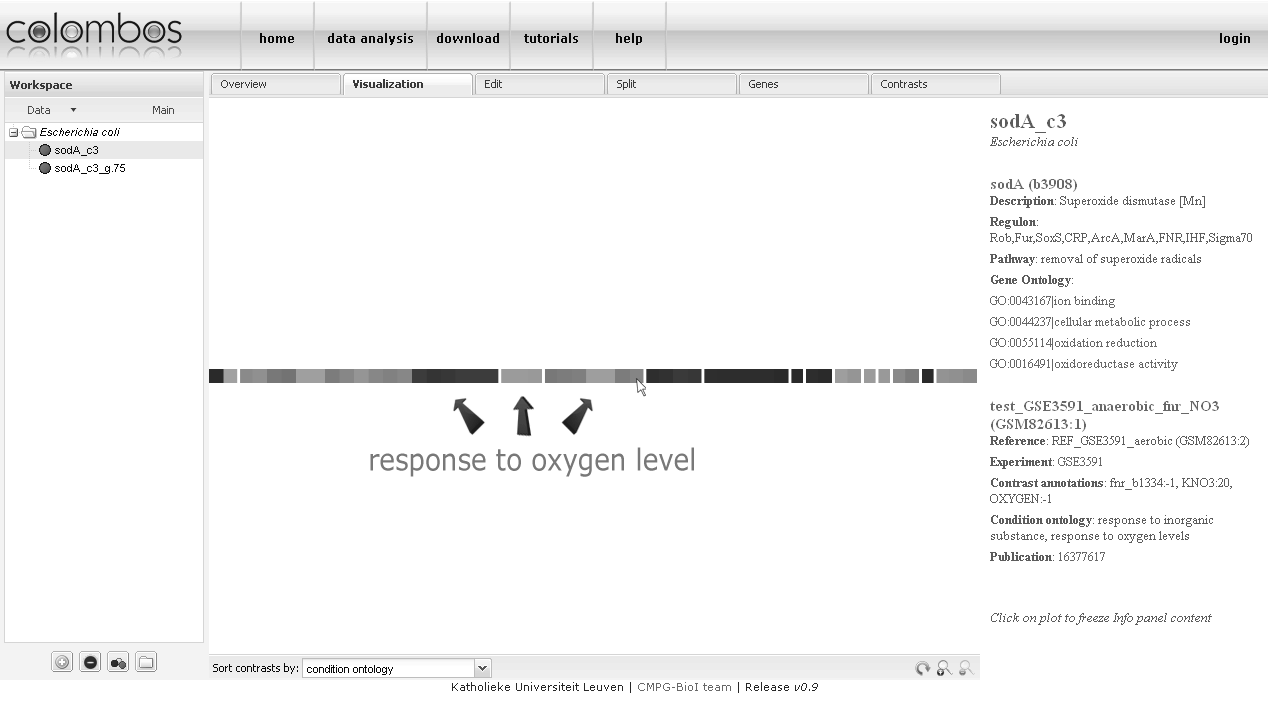
\includegraphics[width=1\textwidth]{Fig6-Heatmap-module-1-white.png}
	\caption[Heatmap of module `sodA\_c3']{\textbf{The visualization tab of 
	module `sodA\_c3' showing the heatmap.}
	In this heatmap, the contrasts are grouped by their ontology annotations. 
	The groups belonging to the ontology term `response to oxygen 
	level' are marked out.}
	\label{fig:colombos-heatmap-m1}
\end{figure}

\end{small} % Step 2

Checking module `sodA\_c3', it shows that the top 53 contrasts, where \textit{sodA} is most differentially expressed, have been selected. Among those, 34 contrasts belong to the condition ontology term `response to oxygen levels'.  It includes condition properties that are linked to cellular processes dependent on oxygen availability, such as \textit{fnr} mutations (a global oxygen responsive transcriptional regulator), NO$_2$ (electron transport decoupler), agitation of the growth medium, actual oxygen levels, etc. This is expected as the function of \textit{sodA} is linked to processes related to oxygen availability. COLOMBOS indeed successfully identifies them as the most relevant contrasts of \textit{sodA}.  There are also 17 contrasts belong to ontology term `growth', with three in common with the aforementioned 34 contrasts. The term `growth' is very general, grouping conditions that trigger various biological processes simultaneously at a global cellular scale. Hence it is not unexpected to find \textit{sodA} differentially expressed under these contrasts.





\subsubsection{Extend the genes of a module}

\begin{figure}[b]
	\centering
  	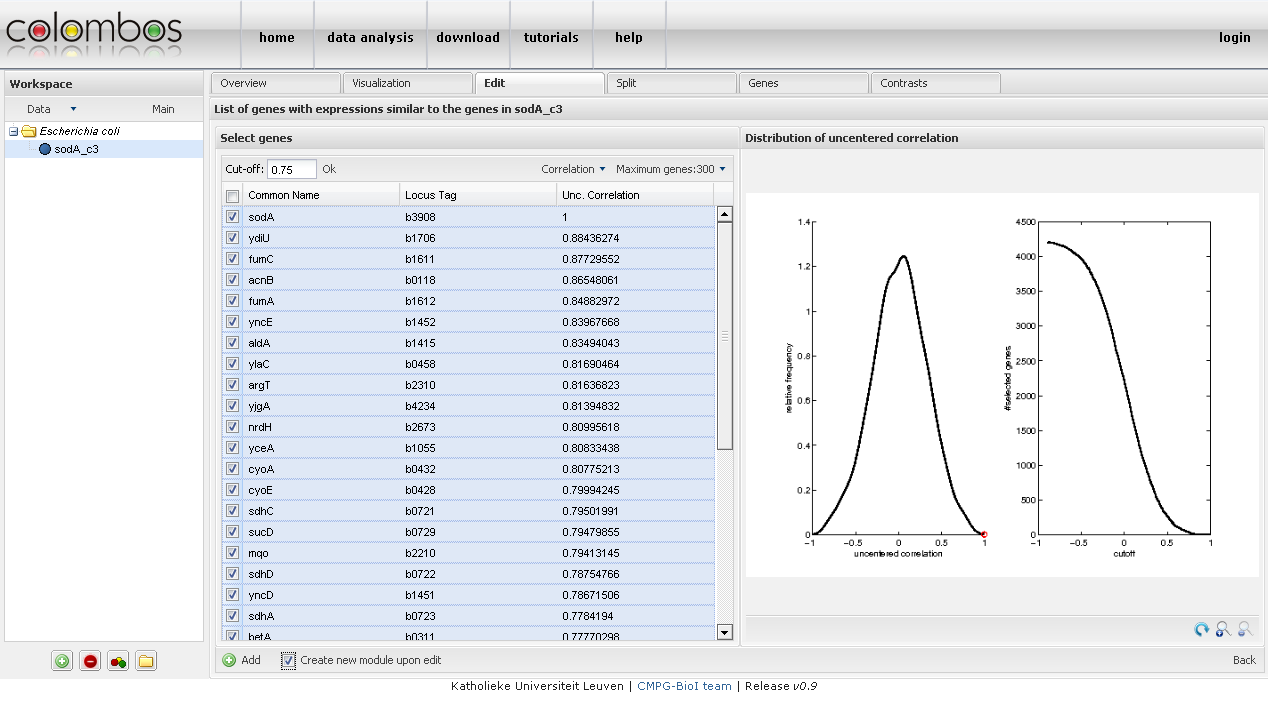
\includegraphics[width=1\textwidth]{Fig7-Gene-extending-panel.png}
	\caption[COLOMBOS `ranked gene selection' interface]{
	\textbf{The `ranked gene selection' interface to extend module `sodA\_c3' 
	with the most relevant genes.} 
	The red circle indicates \textit{sodA} in the module. As it's expression 
	profile is perfectly correlated with itself (the correlation score of 1), 
	the circle is located at point (1, 0).}
	\label{fig:colombos-gene-extend}
\end{figure}

\begin{small} % Step 3


\paragraph{Step 3} Next, we will extend the module with additional genes. Click `edit module' button to go to the `Edit' tab, where three options are available: edit the name/description, the genes, or the contrasts. Click `edit genes' to modify the module genes. A gene modification panel appears with all options to edit genes.  The options in green boxes indicate ways to add genes to the module, whereas those in red boxes indicate ways to remove genes.  For this case study, we will use the last option `Add new genes based on expression' to add additional genes, whose expression patterns are most (anti-)correlated to the expression pattern of the module.  Click it to bring up a `ranked gene selection' panel for gene selection.
\\
This panel (Figure \ref{fig:colombos-gene-extend}) functions in a similar way  to the `ranked contrast selection' panel explained in Step 1.3.  On the left side, a gene list ranked by the degree of the correlation of each gene's expression profile with the mean profile of the module genes under the selected contrasts belonging to this module.   Different types of correlation scores are available to rank the genes. Interested user can refer Appendix \ref{apd:gene-score} for the detailed explanation of the different options.  Here, the default one, which calculates the \textit{Uncentered Pearson Correlation}, is utilized.  The higher the score, the more similar the profiles are.  Similarly, a cutoff value can be specified to select only those genes with higher scores. Also in the panel, the figures to the right show, from left to right, a density plot displaying the distribution of the correlation scores across all genes in the compendium and a plot showing the number of genes that will be added if a given cutoff is selected. The circles connected by a red vertical line in the density plot indicate the gene(s) that already exists in the current module and its correlation score.

To extend our module, we will use a cutoff value of 0.75. The option `Create new module upon edit' (located below the gene list) is checked, so that a new module is created with the extended gene set and the original one is kept unchanged. When ready, click the `Add' button at left, and specify `sodA\_c3\_g.75' (in the pop-up window that appears) to name the new module.  A new node representing newly created module is added below the original module `sodA\_c3' in the workspace.

\end{small} % Step 3

The resulting module now contains 35 genes with an expression profile similar to that of \textit{sodA} under the selected contrasts (see heatmap, Figure \ref{fig:colombos-heatmap-final}).  Amongst the genes in the module are \textit{cyoA}, \textit{cyoB}, \textit{cyoC}, \textit{cyoE}, subunits of the cytochrome b terminal oxidase complex involved in aerobic respiration \cite{Cotter1992}, \textit{sdhA}, \textit{sdhC}, \textit{sdhD}, encoding the succinate dehydrogenase (SdhCDAB) active during Krebs cycle catalyzing the oxidation of succinate to fumarate under aerobic conditions \cite{Wilde1986}, and \textit{sucA}, \textit{sucB}, \textit{sucC}, \textit{sucD} involved in generating succinyl-CoA, one of the reactants in the Krebs cycle \cite{Buck1989}. Considering the functions of these gene products (enriched GO terms in Table \ref{tab:GOenrich}), it is not at all unexpected that their expression levels are influenced by oxygen availability.  Moreover, many genes in module `sodA\_c3\_g.75' also share common regulators with \textit{sodA}, such as ArcA, Fur, FNR, CRP, etc. Hence, \textit{sodA} (encoding a superoxide dismutase activity) being coexpressed with the genes involved in aerobic respiration might be essential to protect the cell against oxidative stress.

\begin{figure}[tb]
	\centering
  	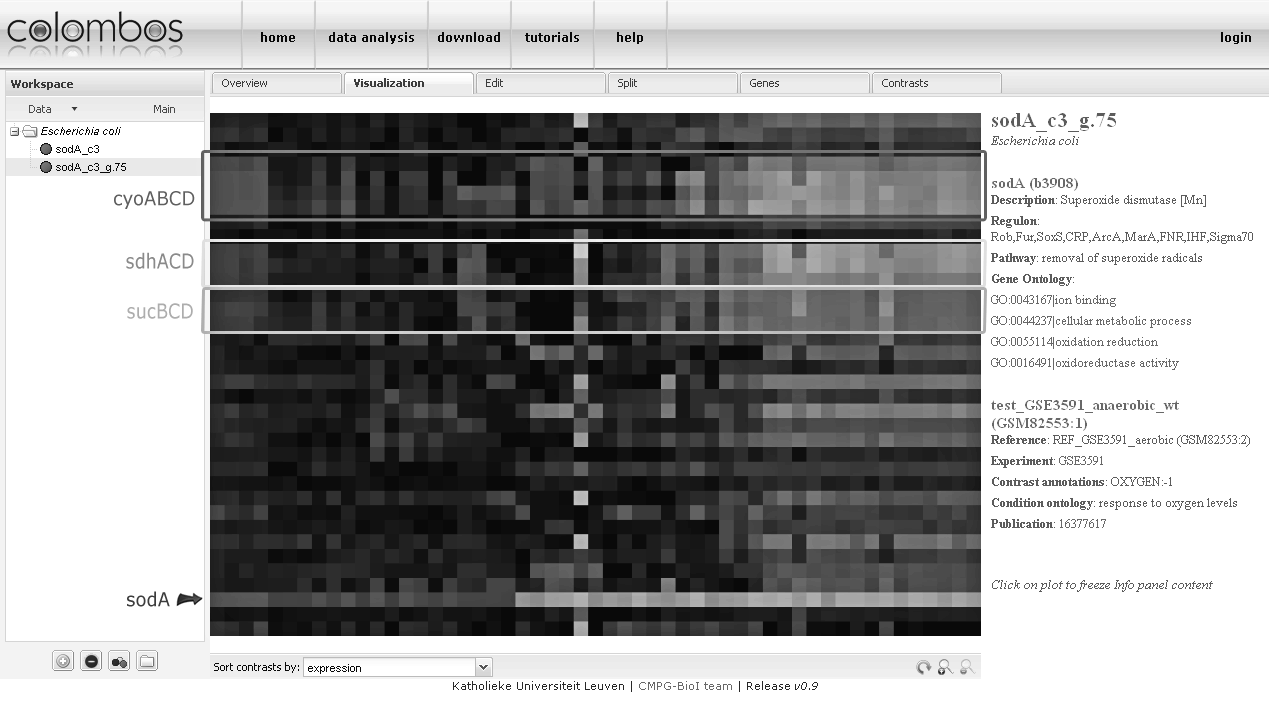
\includegraphics[width=1\textwidth]{Fig8-Heatmap-final-module-tuned.png}
	\caption[COLOMBOS heatmap of module `sodA\_c3\_g.75']{
	\textbf{The heatmap of AU2 module `sodA\_c3\_g.75'.}
	The row of expression data that corresponds to \textit{sodA} is
	marked by the arrow. The expression data of the gene groups that are 
	prominently coexpressed with \textit{sodA}, namely cyoABCD, sdhACD and 
	sucBCD, are marked by the named boxes.}
	\label{fig:colombos-heatmap-final}
\end{figure}


\subsubsection{Summary}

The biological relevance between genes and contrasts of module `sodA\_c3\_g.75' clearly shows the strength of the simple methods implemented in COLOMBOS. Although the coexpression of module genes does not necessarily imply coregulation of its genes,  the promoter regions of these genes could be investigated further using motif detection methods to discover common regulators (see Figure \ref{fig:workflow-distiller-colombos}). This task could be achieved either by screening these regions with Position Specific Scoring Matrices (PSSMs) of previously characterized motifs, or by using \textit{de novo} motif detection methods \cite{Tompa2005, Storms2010}. Moreover that some genes in the module are unannotated, this shows that COLOMBOS web service can also serve as a tool to help biologists identify interesting research candidates.




\subsection{Identifying transcriptional modules with DISTILLER}

DISTILLER \cite{Lemmens2009} is a data integration framework that automatically identifies condition dependent transcriptional modules by combining expression data with information on the interaction between a regulator and its corresponding target genes (here through motif data). Here, we will first show how to setup the related parameters and run each of the three steps of DISTILLER through our web service \cite{DISTILLER}. Then after transcriptional modules are obtained, they are visualized together with the motif information in an interactive way using software ViTraM \cite{Sun2009}. At last, we briefly discuss those resulting modules containing \textit{sodA}.

\subsubsection{Part.1 Running DISTILLER algorithm}\label{sec:dist-distmodule}

DISTILLER automatically identifies all regulatory modules met certain criterion from the expression and motif data of all genes of the species. The target specific ones can then be filtered out from the resulting modules. In this case study, we will use DISTILLER to identify those modules containing \textit{sodA}. Consequently, we can simplify the motif data by removing motifs irrelevant to the query genes.  This greatly reduces the running time of DISTILLER.  After this simplification, only 7 motifs (ArcA, Rob, SoxS, Fur, IHF, FNR, MarA, and CRP) remain.



\paragraph{Create a user profile and a project}
DISTILLER algorithm is computationally expensive, as it explores the complete search space. Depending on the specified parameters and the dataset size, each step could take hours or days to finish.   Consequently, a registration is required, which creates an account with minimally user's email information.  This provides great flexibility, as user can simply setup the system to run a step of the algorithm and leave the site. When process finished, user is notified by an email (details in Section \ref{sec:distiller-email}).  He can then log in and select the corresponding project to continue.



\begin{small} % Step 1,2,3 

\subparagraph{Step 1}	Go to the DISTILLER web service \cite{DISTILLER}.  A new user can be created in three steps, click the `New User' button, complete the required information, and click the `Create User' button.  The user's email address is required for sending notification emails (see Section \ref{sec:distiller-email}).

\subparagraph{Step 2}	After log in, the project selection interface will appear, where one can either select an existing project to continue, or create a new one by clicking `Create New Project' and giving a name and a brief description for it. Here, we create a new project named `Ecoli\_sodA'.  

\subparagraph{Step 3}	After choosing or creating a project, the DISTILLER  panel will appear where the user can run the three main steps of DISTILLER, each of which has its own separate tab. For a new project, only the `Module Detection' tab is accessible (Figure \ref{fig:distiller}), while the `Module Filtering' and `Module Extension' tabs are disabled.

\end{small} % Step 1,2,3 



\paragraph{Identifying seed modules}

\begin{small} % Step 4,5,6
\subparagraph{Step 4} For a new project, user need to first upload the required expression data file and motif data file (see Section \ref{sec:distiller-infile-format}) to be analyzed by DISTILLER program, and preprocess them to check their format and integrity.  As the system supports expression data file in different formats and compression types, it is user's responsibility to specify the correct options for the `Compression' and `Data file format' items in the `Expression Data Parameters' section. Here, the sample files, expdata\_DISTILLER\_Expression.txt and binary\_DISTILLER\_Motif.txt, are used.  Upload them using data file specific upload buttons, specify `Flat file format' as `Data file format' and `No' for `Compression', then click the `Preprocessing' button to start the process on the server. As it is time consuming, the user will be notified by email when the process is done.


\subparagraph{Step 5} After receiving the notification email, user can go back to their project at DISTILLER site.  The interface is the same as seen in Step 4. Only now the button `Run Distiller' is unlocked.  Three groups of parameters need to be specified before starting the process: the binary data parameters for the motif data (see Step 5.1), the expression data parameters (see Step 5.2), and the general ones (see Step 5.3).

\subparagraph{Step 5.1} Binary data parameters: 1) `Binary Support' specifies the minimal number of motifs that the genes in a module should have in common; 2) `Binary Thresholds' is the minimal score a motif instance in the promoter region of a gene should have to be considered as present.   As DISTILLER only accepts binary motif data as input, whereas most motif detection algorithms generate probabilities scoring the certainty of motif gene relations, the specified threshold is applied on the motif data to convert the \textit{continuous values} into the \textit{binary ones}. For this case study, we choose 1 for the Binary Support and  0.999 as the Binary Threshold. Hence the genes belonging to a module must share  at least 1 motif and a gene is considered to have a specific motif if the  corresponding value in the motif data is equal or higher than 0.999.

\subparagraph{Step 5.2}	Expression data parameters: 1) `Box Support' specifies the minimal number of condition contrasts under which the genes in a module should be coexpressed; 2) `Box P-value' is used to generate the threshold bandwidth sequence that is needed to test whether a module passes the constraints on the expression data, i.e. whether the genes in the module are sufficiently coexpressed within the selected contrasts \cite{Lemmens2009}. Here, 100 are chosen for the `Box Support' and 0.0001 for the `Box P-values'.

\subparagraph{Step 5.3} General parameters: 1) `Minimal Module Size' specifies  the minimal number of genes that should be in a module; 2) `Number of Randomizations' specifies the number of random modules that will be generated for computing a threshold bandwidth sequence for the condition contrast selection.  Here, we specify 4 and 10000 for these two parameters respectively. These require that the algorithm generates 10000 random modules consisting of 4 genes to compute the threshold bandwidth sequence.

\subparagraph{Step 6} When all parameters are specified, click `Run Distiller'. DISTILLER will now enumerate all initial modules, each of which contains at least 4 genes coexpressed in more than 100 contrasts and sharing at least one motif. Note these contrasts are selected based on comparing the ordered contrasts bandwidth sequences of given genes with the threshold bandwidth sequence (see \cite{Lemmens2009} for details). When finished, user will receive a notification email (see Section  \ref{sec:distiller-email}) containing the link to the output file with the identified modules, and the link to the supplementary file bundle that is  required to visualize modules using ViTraM. 

\end{small} % Step 4,5,6


\paragraph{Filter the raw DISTILLER output} After obtaining the initial modules, the user can go back to the saved project at DISTILLER site.  Now, the tabs `Module Filtering' and the tab `Module Extending' are enabled.  Note that the user can directly proceed to the module extending step, but due to the discussion in Section \ref{sec:dist-distiller}, performing a filtering step before extending the obtained modules is highly recommended.

\begin{small} % Step 7
\subparagraph{Step 7} Click the `Filtering' tab, specify the number of modules to be filtered out in this step, then click on `Filter Result' to proceed.  In our case study, the top 20 modules ranked by their scores computed by DISTILLER are selected (see Section \ref{sec:dist-distiller}). Similarly, the result of the process will be notified by email.

\end{small}

\paragraph{Extend DISTILLER seed modules} After obtaining the filtered results, the user can now proceed with the `Module Extension' step. In this step, extra genes are incorporated into a module if they comply with the relaxed criteria.

\begin{small} % Step 8,9,10

\subparagraph{Step 8} Two parameters need to be specified to run this step. Candidate genes have to comply with both parameters in order to be included in the extended module. The only exception is made for the genes belong to an \textit{operon} (see Step 9). 

\subparagraph{Step 8.1} `Extended Motif Threshold': this is the same type of parameter as the `Binary Thresholds' specified in Step 5.1, but less stringent to allow a gene having more present motifs. As a result, more genes can satisfy the `Binary Support' parameter.  Here, we use 0.95 for this parameter (as compared to 0.999 for the `Binary Thresholds').

\subparagraph{Step 8.2}	`Correlation Percentage': a correlation threshold to select candidate genes for module extension.  Given a `Correlation Percentage' of $p$, only those genes whose expression profile correlations, calculated based on the mean expression profile of a module, higher than $p$, are considered as the candidates. Here we choose $p$ as 0.95.


\subparagraph{Step 9} Optionally, the genes of a module can be further extended with \textit{operon information} if available.  Candidate genes belonging to an operon, whose first gene is present in a seed module, only need to satisfy the criterion for the expression profile (`Correlation Percentage') to be included into the module.  The operon information (i.e. which genes belong to which operon) is included in the analysis by uploading a file containing the corresponding data (see Section \ref{sec:distiller-infile-format}). 

\subparagraph{Step 10} After specifying the parameters and optionally uploading an operon data file, the user can click `Extend Modules' to run the process.  A notification email is sent when the process is finished.

\end{small} % Step 8,9,10

After receiving the final output file of DISTILLER, the user can then specifically select the modules that contain his or her query genes, in our case the gene \textit{sodA}, to continue.





\subsubsection{Part.2 Visualization of DISTILLER modules with ViTraM}
The software ViTraM is used to analyse modules discovered by DISTILLER. However, the DISTILLER output files need to be converted into ViTraM compatible format first.  Then, ViTraM can be utilized to visualize the modules.

DISTILLER is non-deterministic due to the randomization process utilized by the algorithm to select contrasts. Thus, it is possible that when following exactly the same way as outlined here to run DISTILLER, the recovered modules are different from those obtained in this example (as provided in `DISTILLER\_outputExtended.m' sample file, see Section \ref{sec:dist-sample}).  Use the corresponding sample file to proceed with exactly the same results.


\paragraph{Prepare ViTraM readable files}

\begin{small} % Step 1,2 ViTraM
\subparagraph{Step 1} Download the XMLCreator from the ViTraM website\cite{ViTraM} and unzip the file. Under linux, run the XMLCreator by typing the command `java -jar -Xms256m -Xmx512m XMLCreator.jar' in a terminal.  Windows users can click file `XMLCreator\_Windows\_512M.bat' to run it.

\subparagraph{Step 2} In the pop-up window, choose `DISTILLER' as module detection tool and click on `OK'.   The main interface appears where user can specify the input and output files. Two required input files are the DISTILLER `.m' output data file and the `Expression Data' file (see Section \ref{sec:dist-vitram}).  In addition, other files providing extra information can be visualized along with the modules. This includes but not limited to, the motif information of each gene, the genes' functional annotations, or the experimental factors and/or sample characters of each , etc. Finally, the names of the output files need to be specified. Two output files will be generated: the module XML file and the corresponding expression data file containing the expression values for those genes and contrasts presented in any of the modules. 

\end{small} % Step 1,2 ViTraM

Here, we demonstrate this step using the corresponding sample files, the `DISTILLER\_outputExtended.m' and the `expdata\_DISTILLER\_supple.txt'. Additionally, the file `binary\_DISTILLER\_Motif\_supple.txt' providing extra motif information for each module is specified as the `Motif Data'. We then run XMLCreator to generate the two output files, `ViTraM\_Modules.XML' and `ViTraM\_Expression.txt'. To run XMLCreator on the DISTILLER output, pleases always use the supplement files specified in the notification email that accompanies the `.m' file (see Section \ref{sec:distiller-email}).


\paragraph{Run ViTraM}

From the ViTraM website \cite{ViTraM}, the user can  download ViTraM v2.0 and unzip the file. Note, a registration is required by  providing us some basic information, and the user must accept our software  license.

\begin{small} % Step 3-10 ViTraM

\subparagraph{Step 3} To run ViTraM under windows, click on  `ViTraM\_Windows\_512M.bat' or `ViTraM\_Windows\_2G.bat' provided.  The latter can handle larger datasets, but does require more than 2Gb physical memory in the computer. To run ViTraM under linux or mac, call `ViTraM\_Linux\&Mac.sh' file.

\subparagraph{Step 4} Load `ViTraM\_Modules.XML' and `ViTraM\_Expression.txt'  generated in Step 2 by operations `Open Module XML File' and `Open Expression File' in the 'Input' panel respectively.  After the data are loaded, they can be visualized by `Load All Modules' in the `Module Selection' panel.  This extra loading step enables visualizing a subset of modules, where directly visualizing all the modules in a large dataset generally causes memory issues. In such a case, user can use `Filter' panel first to select only the relevant modules, then visualize them. This significantly reduces the loading time to visualize modules.

\subparagraph{Step 5} Subsequently click on `View Modules' in the  `Module Display' panel to show the modules in the main window.  In this window, the genes are listed at the left and the conditions at the top, and each module is represented as one or a group of boxes with its id shown at the top left corner of each box and a distinctive color for each module.

\subparagraph{Step 6} Click `View Gene Properties' in `Gene Properties  Display' panel, the extra properties of the gene can be visualized together with the modules in an extra window located at the left side of the `Module Display' window.  The motif information provided in Step 2 will now appear here. The color of each cubic represents the value of the motif score explained in Section \ref{sec:dist-vitram}.  The red color corresponds to the high value and the green the low one. If a score is higher than a threshold, a cross will appear in the corresponding cubic.


\subparagraph{Step 7} By clicking on `Favorite Genes' in the `Filter' panel  at the right hand side, it is possible to display only those modules containing a particular gene. The pop-up window shows on the left a list of all genes. Select the gene `b3908' (\textit{sodA}), and click the arrow button `\textrightarrow' to add it to the favorite gene list at the right.  Then click `OK'.  Only modules containing \textit{sodA} will still be in display.

\subparagraph{Step 8} To optimize the visualization of modules that overlap,  click on `Automatic ordering' in the `Module ordering' panel and subsequently `Run Overlap Index' to layout the currently displayed modules in the most optimal way (for details on the algorithms that identify the optimal display of overlapping modules, we refer to \cite{Sun2009}).

\subparagraph{Step 9} Click on `View Modules' and subsequently `Refresh  Modules' in the `Overview \& Heatmap Display'. Then click on `Adding Heatmap'.  The expression values of the genes for the condition contrasts in the currently  displayed modules will be shown by means of a heatmap.

\end{small} % Step 3-10 ViTraM


\subsubsection{Analyzing resulting DISTILLER modules containing \textit{sodA}}

In this case study, we used DISTILLER to search for modules of coexpressed genes sharing at least one motif instances for the same regulator.  Resulting modules including the motif instances shared among genes within each module are listed in Table \ref{tab:distModules}.  Since we are interested in \textit{sodA}, transcriptional modules 2, 3, 8, and 12 containing this gene were selected and visualized using ViTraM (Figure \ref{fig:vitram}).   The numbering of the modules corresponds to their ranks in the filtered results. Note that as a global method, DISTILLER identifies all possible regulatory modules in the dataset (not only those with \textit{sodA}). So the numbering of the modules containing \textit{sodA} is not consecutive. The lower the number, the more significant a module is.

\begin{figure}[b]
	\centering
  	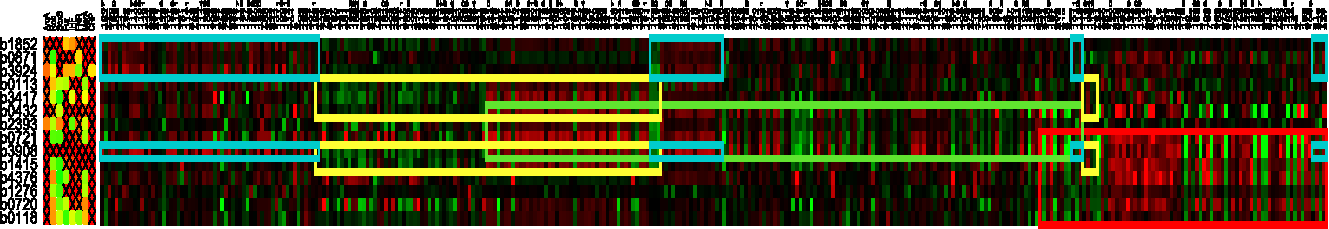
\includegraphics[width=1\textwidth]{Fig9-Distiller-modules-color.pdf}
	\caption[DISTILLER \textit{sodA} related modules visualized in ViTraM] 
	{\textbf{DISTILLER \textit{sodA} related modules visualized in ViTraM.}
	The figure shows the four modules containing \textit{sodA}. Each module is 
	indicated with one or more squares and expression values are indicated by 
	heatmap. Module 2 is indicated by blue lines, module 3 by red line, 
	module 8 by green lines, and module 12 by yellow lines.}
	\label{fig:vitram}
\end{figure}

\begin{table}[tb]
	\caption{Overview of the 20 transcriptional modules identified by DISTILLER}
	\label{tab:distModules}
	\begin{small}
	\begin{tabular}{p{5mm} p{2cm} c c p{4.5cm}}
	\toprule
	{\bf ID} & {\bf Motifs} & {\bf \# Genes} & {\bf \# Conds} & {\bf Genes in 
	\textit{sodA} modules} \\
	\midrule
	1 & Fur	& 22 & 97 & \\
	2 &	MarA, SoxS & 4 & 77	& \textit{fpr}, \textit{poxB}, 	
	\textit{\textbf{sodA}}, \textit{zwf} \\
	3 &	ArcA, CRP &	7 &	79 & \textit{acnA}, \textit{acnB}, \textit{aldA}, 
	\textit{gltA}, \textit{osmY}, \textit{sdhC}, \textit{\textbf{sodA}} \\
	4 &	FNR, IHF & 4 & 226 & \\
	5 &	ArcA, FNR &	4 &	123	& \\	
	6 &	CRP	& 308 &	107	& \\
	7 &	CRP, FNR & 4 & 87 & \\
	8 &	Fur, CRP & 4 & 146 & \textit{cyoA}, \textit{nupC}, \textit{sdhC}, 
	\textit{\textbf{sodA}} \\
	9 &	SoxS & 4 &	181	& \\
	10 & Fur & 18 & 86	& \\
	11 & MarA &	4 &	206	& \\
	12 & CRP, FNR & 5 &	90 & \textit{aldA}, \textit{cyoA}, 
	\textit{malP}, \textit{pdhR}, \textit{\textbf{sodA}} \\
	13 & IHF &	8 &	87	& \\
	14 & IHF &	53 & 123	& \\
	15 & FNR &	38 & 102	& \\
	16 & CRP &	76 & 125	& \\
	17 & ArcA, CRP &  4 &	148	& \\
	18 & SoxS &	4 &	95	& \\
	19 & Fur & 4 &	100	& \\
	20 & Fur & 22 &	76 & \\
	\bottomrule
	\end{tabular}
	\end{small}
\end{table}

\begin{table}[tb]
\begin{threeparttable}
	\caption{GO enrichment of \textit{sodA} modules\tnote{1}}
	\label{tab:GOenrich}
	\begin{small}
	\begin{tabular}{p{2.2cm} c c p{5.3cm}}
	\toprule
	{\bf Module} & {\bf P-value} & {\bf GO ID} & {\bf GO Term Description} \\
	\midrule
	{\bf\it COLOMBOS} \\
	\hline
	\textit{sodA\_c3\_g.75}	& 2.41e-12 & GO:0006091 & generation of precursor 
	metabolites and energy \\
	& 9.23e-02 & GO:0006800 & oxygen and reactive oxygen species metabolic 
		process \\
	& 3.17e-02 & GO:0006869 & lipid transport \\
	& 2.74e-07&	GO:0022900&	electron transport chain \\
	& 4.22e-02&	GO:0042592&	homeostatic process \\	
	& 1.85e-02&	GO:0045454&	cell redox homeostasis \\[2ex]
	{\bf\it DISTILLER} \\
	\hline
	\textit{module2} & 7.07e-02&	GO:0005996&	monosaccharide metabolic 
	process \\
	& 7.11e-03&	GO:0006800&	oxygen and reactive oxygen species metabolic 
		process \\
	\hline
	\textit{module3} & 3.11e-05&	GO:0006091& generation of precursor 
	metabolites 
	and energy \\
	& 1.77e-02&	GO:0006800&	oxygen and reactive oxygen species metabolic 
	process \\
	& 7.11e-02&	GO:0044262&	cellular carbohydrate metabolic process \\
	\hline
	\textit{module8} & 4.09e-03&	GO:0006091&	generation of precursor 
	metabolites 
	and energy \\
	& 1.06e-02&	GO:0006800&	oxygen and reactive oxygen species metabolic 
	process \\
	& 4.09e-03&	GO:0022900&	electron transport chain \\
	\hline
	\textit{module12}& 1.42e-02& GO:0006800& oxygen and reactive oxygen 
	species metabolic process \\
	\bottomrule
	\end{tabular}
	\begin{tablenotes}
	\item[1] Enriched GO terms are ordered by GO access ID.
	\end{tablenotes}
	\end{small}
\end{threeparttable}
\end{table}


Module 2 contains the genes regulated by both SoxS and MarA. The identified contrasts in this module belong to the ontology terms `carbohydrate metabolic process', `growth', and `response to oxidative stress'. SoxS and MarA are known to participate in the removal of superoxide and nitric oxide and protection from organic solvents \cite{Touati2000}.  One can expect that the contrasts belonging to `response to oxidative stress' to be suitable for inducing their expression and therefore the expression of genes regulated by them.  We already highlighted the link between the removal of superoxide species and metabolic pathways.  It explains why the condition contrasts under `carbohydrate metabolic process' are found in this module.   As discussed after Step 3 of Section \ref{sec:dist-module-colombos}, to observe condition contrasts belonging to `growth' is not unreasonable in this case.   In addition to \textit{sodA}, the other genes found in this module are \textit{fpr} (Ferredoxin-NADP reductase), \textit{poxB} (Pyruvate dehydrogenase), and \textit{zwf} (Glucose-6-phosphate 1-dehydrogenase). The enriched GO terms of this gene set (Table \ref{tab:GOenrich}) are highly consistent with the observed condition ontology terms.


In module 3, genes are regulated by both ArcA and CRP. Its condition contrasts are highly related to the ontology terms `growth' and `response to oxygen levels'.  CRP is a global regulator involves in the degradation of any non-glucose carbon sources and also an antagonist of catabolite repression.  On the other hand, ArcA participates specifically in a signal transduction system sensing particular aerobic and anaerobic growth conditions \cite{Compan1994}.   The functions of the genes found in this module (\textit{acnA}, \textit{acnB}, \textit{aldA}, \textit{gltA}, \textit{osmY}, \textit{sdhC}, and \textit{sodA}) are an intersection between global metabolic pathways and specific processes responding to oxygen level changes (see Table \ref{tab:GOenrich}).


Genes in module 8 are both regulated by CRP and Fur. As previously mentioned, CRP is a global regulator that facilitates bacterial fitness in function of the availability of different carbon sources.  Fur is a sensor of intercellular iron concentration, and also participates in the response to reactive nitrogen species \cite{Mukhopadhyay2004}.   The contrasts of this module mainly involve `carbohydrate metabolic process', `growth', `detoxification of nitrogen compound', `lactose catabolic process'.  Except for \textit{sodA}, the genes found in this module are \textit{cyoA} (Ubiquinol oxidase subunit 2), \textit{nupC} (Nucleoside permease nupC), and \textit{sdhC} (Succinate dehydrogenase cytochrome b$_{556}$ subunit). Altogether the condition contrasts and the genes selected in this module reflect the linkage between basic metabolism changes induced by external C-source availability (e.g. glucose concentration) and intra-cellular energy production through the electron transfer chain (see also enriched GO terms in Table \ref{tab:GOenrich}).


In module 12, genes are regulated by CRP and FNR, both master-regulators.  FNR activates genes involved in anaerobic metabolism and represses genes involved in aerobic metabolism.  The enriched GO term (only `oxygen and reactive oxygen species metabolic process') for this module's gene set reflect this. The selected contrasts of this module constitute a very broad set of ontology terms, including `carbohydrate metabolic process', `growth', `dna repair', `sos response', `lactose catabolic process', and `detoxification of nitrogen compound'.  This is in line with the global regulation exerted by CRP and FNR.


\section{Discussion and Conclusion}

The COLOMBOS web service provides very straightforward and intuitive ways for analyzing and exploring large-scale expression compendia. It is intended for specific queries based on users pre-knowledge on genes or conditions of interest. In each step, this knowledge and user involvement is crucial to explore various functionalities in order to generate good quality results.  It is a deterministic approach, which means that when executing exactly the same operations, COLOMBOS will generate exactly the same result. Furthermore, the analysis methods implemented in COLOMBOS are fast, generally taking only seconds or less to generate results for each step.

DISTILLER, on the other hand, is a semi-automatic method. Except for a limited set of parameters, it requires very little user involvement. Guided by both motif information and expression data, the method tries to compose a global regulatory network that covers the whole input dataset (see Table \ref{tab:distModules}). It is non-deterministic due to the randomization involved in generating a threshold bandwidth sequence for the condition selection (see Step 8 in Section \ref{sec:dist-distmodule}).

In this case study, we have used COLOMBOS and DISTILLER to gain insights in the functional processes, in which \textit{sodA} is involved, and the regulatory programs that coordinate them. This resulted in one module identified by COLOMBOS and four modules by DISTILLER.  As discussed in previous sections, each module does reflect relevant biological processes, in which genes including \textit{sodA} participate.  This does not necessarily require the modules to overlap, as each might represent different processes involving different genes.  When these two approaches are used to address the same biological question as was done here, the distinct features of each approach lead to different but meaningful and thus complementary results.

The module `sodA\_c3\_g.75' identified by COLOMBOS contains several genes involved in various biological processes (see Figure \ref{fig:colombos-heatmap-m1} and the discussion at the end of Section \ref{sec:dist-module-colombos}) with very high and coherent expression values under most contrasts (in both cases where up-regulation or down-regulation occurred). In contrast, when compared to module `sodA\_c3\_g.75', each of the DISTILLER modules contains in general much less genes, which show less extreme expression levels indicating a weaker coexpression signal compared to `sodA\_c3\_g.75'.

When evaluating the overlap between modules found by these two methods, module 3 and `sodA\_c3\_g.75' share four genes (\textit{aldA}, \textit{acnB}, \textit{sdhC}, \textit{sodA}) and 19 contrasts (`response to oxygen level', `growth').  These contrasts represent approximately 25\% and 35\% of all condition contrasts of each module respectively. Module 8 and `sodA\_c3\_g.75' have three genes (\textit{cyoA}, \textit{sdhC}, \textit{sodA}) and eight condition contrasts (`response to oxygen level') in common, which represent approximately 6\% and 15\% of all condition contrasts in each module.  This kind of similarity can be expected, since we applied both methods to answer same biological question based on the same expression data.

On the other hand, no overlap is observed between module 2 and `sodA\_c3\_g.75'.  Module 12 shares three genes (\textit{aldA}, \textit{cyoA}, \textit{sodA}) with `sodA\_c3\_g.75' though, but the two modules have no contrasts in common.  Upon closer inspection of the expression data, genes in DISTILLER module 2 are coexpressed, but the expression value of \textit{sodA} is not very high for these contrasts, when compared with those of `sodA\_c3\_g.75'. Hence those contrasts will not be easily picked up by COLOMBOS in Step 2.3 of Section \ref{sec:dist-module-colombos} (unless a much lower selection threshold is used).  Furthermore, genes appearing only in the DISTILLER modules show a different expression behavior from that of \textit{sodA} under those contrasts selected by COLOMBOS.  As a result, when extending genes of a module based on expression profiles (see Step 4 of Section \ref{sec:dist-module-colombos}), those genes will be ranked less relevant. Consequently, they will hardly be considered as prime candidates for module extension.

In summary, COLOMBOS focuses on using expression values as its main criterion for building modules, resulting in clear expression changes in tight coexpression. It can easily extract prominent coexpression behaviour in the expression data, but might miss modules with less significant coexpression patterns. The coexpression patterns retrieved by COLOMBOS can be broadly interpreted as genes being functionally related as their abundance are altered in similar ways in response to various stimuli. This functional relationship could imply coregulation (which might be identified using motif detection algorithms, see also Figure \ref{fig:workflow-distiller-colombos}), but it is not a necessary prerequisite. Instead, it cannot be excluded that several regulatory programs might be  responsible for the observed coexpression patterns. On the other hand, DISTILLER, as a global method, tries to recover distinctive modules that can be directly linked to a shared regulatory program, i.e. of which the genes are coregulated by the same (set of) regulator(s). Combining motif information with expression data, it successfully retrieves less prominent coexpression patterns with biological significance by utilizing extra information regarding the presence (or prediction, depending on the nature of the motif input data) of transcription factor binding sites in its genes promoter regions. The case study of \textit{sodA} presented in this chapter illustrates  this complementarity of these two approaches for retrieving biologically  relevant results. 

In this chapter, we focus on the specific application of the COLOMBOS and DISTILLER.  However, versatile tools as them have many other functionalities and application domains. In COLOMBOS, various options exist to build the module based on the information other than a given set of genes.  Furthermore, if desirable, the module data can be downloaded for further analysis.  As an example, the data of the module `sodA\_c3\_g.75' is exported into file `expdata\_COLOMBOS\_module\_information.txt' (available as a sample file, see Section \ref{sec:dist-sample}). DISTILLER can use other data sources as input, for instance, the information  on the binding of regulators as obtained from ChIP-chip experiments  \cite{Lemmens2009, Lemmens2006}. Furthermore, it can be used together with data source other than motif data to  discover other type of networks, as long as connections exist between the data  source and the gene expression profile.  Two such example data sets are protein-protein interaction data or synthetic lethality data.



%%%%%%%%%%%%%%%%%%%%%%%%%%%%%%%%%%%%%%%%%%%%%%%%%%
% Keep the following \cleardoublepage at the end of this file, 
% otherwise \includeonly includes empty pages.
\cleardoublepage
 
% vim: tw=70 nocindent expandtab foldmethod=marker foldmarker={{{}{,}{}}}
